\documentclass[12pt,a4paper,ngerman]{article}
\usepackage{ifpdf}
\usepackage[utf8x]{inputenc}
\usepackage[ngerman]{babel}
\usepackage{fancyhdr}
\usepackage[pdftex]{graphicx}
\usepackage{graphicx}
\usepackage{amsfonts}
\usepackage{listings}
\usepackage{wrapfig}
\usepackage{boxedminipage}
\usepackage{color}
\lstset{ %
language=sh,                % choose the language of the code
basicstyle=\scriptsize,       % the size of the fonts that are used for the code
numbers=left,                   % where to put the line-numbers
numberstyle=\scriptsize,      % the size of the fonts that are used for the line-numbers
stepnumber=1,                   % the step between two line-numbers. If it's 1 each line will be numbered
numbersep=5pt,                  % how far the line-numbers are from the code
backgroundcolor=\color{white},  % choose the background color. You must add \usepackage{color}
showspaces=false,               % show spaces adding particular underscores
showstringspaces=false,         % underline spaces within strings
showtabs=false,                 % show tabs within strings adding particular underscores
%extendedchars=false,
frame=single,			% adds a frame around the code
tabsize=2,			% sets default tabsize to 2 spaces
captionpos=b,			% sets the caption-position to bottom
breaklines=true,		% sets automatic line breaking
breakatwhitespace=false,	% sets if automatic breaks should only happen at whitespace
escapeinside={\%*}{*)}          % if you want to add a comment within your code
}
\usepackage{amsmath}
\usepackage{cancel}
%\usepackage{mathcomp}
%\usepackage{booktabs} 
\usepackage{subfigure}
\usepackage{url}
%\usepackage[document]{ragged2e}

\usepackage[numbers]{natbib}
%\usepackage{tikz}
%\usetikzlibrary{shapes,arrows}

\clubpenalty = 10000
\widowpenalty = 10000 \displaywidowpenalty = 10000
\usepackage[top=2.5cm, bottom=2cm, left=2.5cm, right=2.5cm]{geometry} 
\title{Deliver with Puppet}
\author{Anders Malmborg and Michael Haslgruebler}

\makeatletter
\fancypagestyle {plain}{
  \lhead {}
  \rhead {\@title}
  \cfoot {}
  \lfoot {2012, Anders Malmborg und Michael Haslgrübler}
  \rfoot {\thepage}
  \renewcommand {\footrulewidth }{1pt}
}
\makeatother

%\textwidth17cm
%\textheight24.5cm  
%\textwidth24.5cm
%\textheight17cm  
\headheight15pt

\makeatletter
\ifpdf
\pdfinfo {
	/Author (\@author)
	/Title (\@title)
	/Subject ()
	/Keywords ()
}
\fi
\makeatother


\newcommand{\reffig}[1]{, siehe. Abbildung~\ref{#1}}
\newcommand{\reflst}[1]{, siehe. Listing~\ref{#1}}

\begin{document}
 % meine jabber ID michael (at) jabber.haslgruebler.eu
 \begin{titlepage}
     \begin{flushright}{\huge Deliver with Puppet}
	\end{flushright}
	\hrule
      
      \begin{flushright}
	  {\large Anders Malmborg und Michael Haslgrübler}\\
	  \today
	\end{flushright}
 \end{titlepage}

\pagestyle{plain}

\section{Einleitung}

\subsection{Ausgangssituation}

Eine prekäre Situation, eine mehrere Teams entwickeln, unabhängig voneinander mit agilen Methoden, eine Vielzahl von modularen Frameworks und Applikationen. Mithilfe von \cite{jenkins} wird stündlich kompiliert und integriert um sicherzustellen dass das alles auch zusammenpasst. 

Jede Applikation beinhaltet außerdem Konfigurationen, im banalsten Fall sind das Einstellungen für den Zugriff auf eine Datenbank, im komplexesten Fall Schalter welche Teilfunktionalitäten aktivieren. Die Installation und Konfiguration gestaltet sich aber mit zunehmender Größe der Applikation jedoch so komplex, dass das initiale Setup einer Applikation schon Stunden dauern kann, auch wenn schon eine handvoll Scripts einen Großteil der Tätigkeiten automatisierten. 

\begin{wrapfigure}{l}{5cm}
\vspace{-15pt}
\begin{boxedminipage}{5cm}
Eine Installation von der selben Anwendung sieht auf verschiedenen Maschinen unterschiedlich aus  - \textbf{frei nach dem Motto viele Wege führen nach Rom - aber welcher ist der Beste?}
\end{boxedminipage}
\vspace{-15pt}
\end{wrapfigure}
Man kann außerdem davon ausgehen, das die gleiche Installation von der selben Anwendung auf zwei Rechner unterschiedlich aussieht -- frei nach dem Motto viele Wege führen nach Rom. Zusätzlich dazu sind die Anwendungen im internationalen Einsatz, werden mehrsprachig getestet und betrieben und die laufende Entwicklung erweitert ständig die Funktionalität. 

Kurz zusammengefasst, Veränderungen passieren am laufenden Band. Für die reine Softwareentwicklung ist Continous Integration mit Jenkins und Co eine Toollandschaft entstanden welche das Problem löst. Für die Betriebsführung und Konfiguration haben wir uns nach einer Lösung umgesehen und mit \cite{puppet} und \cite{chef} Wege gefunden dieser ständigen Veränderung habhaft zu werden.

\subsection{Ziel}

Ziel unserer Lösung, für die Betriebsführung und Konfiguration, sollte es sein, die aktuellen Entwicklungen an den Mann bzw. Server zu bringen, vollautomatisiert. 
\begin{wrapfigure}{r}{5cm}
\vspace{-10pt}
\begin{boxedminipage}{5cm}
Konfigurationsfehler durch Divergenz werden in allen Stages des Softwarelifecycleprozesses durch die Vollautomatisierung vermieden - \textbf{entweder funktioniert es überall oder nirgends}
\end{boxedminipage}
\vspace{-10pt}
\end{wrapfigure}
 In der Entwicklung heißt das in erster Linie Softwarecode der commited wird, der gebaut werden kann und die automatisierten Tests besteht soll auch deployed werden. Damit können wir gewährleisten bzw. überprüfen das die Software zu jedem Zeitpunkt einsatzbereit ist und nicht nur auf einem Entwicklungs-PC funktioniert.

Für die Qualitätssicherung heißt das, dass ein Softwarepaket einer Anwendung bei Übergabe von der Entwicklung nur einmal zentral hinterlegt werden muss und alle QA Server in allen möglichen Konfigurationsarten und Sprachen automatisch auf den neusten Stand der Anwendung gebracht werden.

Für den Produktiveinsatz heißt dass das auch hier alle Server auf Knopfdruck aktualisiert werden können und die Server einen definierten und bereits in QA getesten Zustand sind und bleiben. 

Um diese Ziele zu erreichen sind einige Veränderungen notwendig. In diesem Artikel möchten wir uns auf die notwendigen Änderungen im Entwicklungsprozess eingehen und wie wir diese mit Puppet umgesetzt haben.

\section{Entwicklung mit Puppet}

Puppet kann unter für Unix mit einem Paketmanager installiert werden oder für Windows von \cite{puppetlabs} runtergeladen werden. Für die Entwicklung von Puppet Module und Manifeste, mehr dazu später, bietet sich \cite{geppeto} an, welches als Standaloneapplikation installiert werden kann oder in eine bestehende Eclipseinstallation als Plugin hinzugefügt werden kann.

Für die Entwicklung und Tests von Puppet Modulen und Manifeste wird hier \cite{vagrant} verwendet. Vagrant ist eine Konfigurationstool für die Verwaltung von Virtuellen Maschinen mit \cite{virtualbox}. Es kann in weiterer Folge auch Puppet, Chef oder Shell Scripts benutzen kann um die virtuelle Maschine zu konfigurieren. Analog zu Puppet können Vagrant und Virutalbox via Paketmanager für Linux installiert werden oder von den entsprechenden Downloadseiten runtergeladen werden.

\subsection{Testbox mit Vagrant}

\begin{wrapfigure}{l}{5cm}
\vspace{-15pt}
\begin{boxedminipage}{5cm}
Eine Liste mit vorgefertigten Vagrant Boxen gibt es übrigens auf \url{http://www.vagrantbox.es/}
\end{boxedminipage}
\vspace{-15pt}
\end{wrapfigure}

Nachdem Vagrant und VirtualBox installiert worden sind, können wir eine Box zum Testen aufsetzen. In unserem Fall verwenden wir eine 64 Bit Version von Debian Squeeze. Diese wurde von uns für diesen Artikel neu erstellt und beinhaltet eine Minimalinstallation mit den für Vagrant üblichen Vorbereitungen: SSH Key Setup, VirtualBox Guest Additions, Puppet und Ruby. \url{http://vagrantup.com/v1/docs/base_boxes.html}

\begin{lstlisting}[caption=Download der Vagrant Box, label=vagrant-add]
vagrant box add debian_squeeze_64 http://dl.dropbox.com/u/937870/VMs/squeeze64.box
\end{lstlisting}

%\begin{center}
%\fbox{%
\begin{wrapfigure}{r}{4.5cm}
\vspace{-20pt}
%\vskip 3cm
\begin{boxedminipage}{4.5cm}
 Die Vagrant Boxen werden unter Unix in installiert. \lstinline!$HOME/.vagrant.d/boxes!
Falls man dies ändern will kann man die Umgebungsvariable \lstinline$VAGRANT_HOME$ setzen:
\begin{lstlisting}[label=vagrant-home,frame=none,numbers=none]
export VAGRANT_HOME=$HOME/vagrant_home
\end{lstlisting}
\end{boxedminipage}
%\vspace{+30pt}
\vspace{-20pt}
%\vskip 2cm
\end{wrapfigure}
%\end{minipage}}
%\end{center}
%\label{test}
  

Nachdem dem Download steht uns jetzt die  Vagrant Box \lstinline$debian_squeeze_64$ zur Verfügung. Nun können wir in ein beliebiges Verzeichnis wechsel und eine initiale Konfiguration basierend auf der Box anlegen\reflst{vagrant-init}.

\begin{lstlisting}[caption=Vagrant initialisieren, label=vagrant-init]
vagrant init debian_squeeze_64
\end{lstlisting}

Diese initiale Konfiguration beinhaltet alles an was Vagrant zum Konfigurieren und Starten der Maschine braucht, es sind keine weiteren Einstellungen mehr nötig und wir können diese starten\reflst{vagrant-up}.

\begin{lstlisting}[caption=Starten der Vagrant Maschine, label=vagrant-up]
vagrant up
\end{lstlisting}

\subsection{Puppet Einführung}

Puppet benutzt eine Domain-Specific-Language um den Zustand eines System zu beschreiben. Diese Beschreibung wird in einem Manifest festgehalten. Ein Großteil dieser Manifeste mach die Definition von Ressourcen aus, eine Ressource ist ein atomarer Typ eines Systems, es entspricht einer physisches Identität eines Computersystems. Ein Beispiel für eine solche Ressource, wäre ein Benutzer oder eine Datei. Im Beispiel\reffig{puppet-user}, sehen wir wie wir einen Benutzer und eine Datei mit der Puppet DSL anlegen.

\begin{figure}
  \begin{center}
    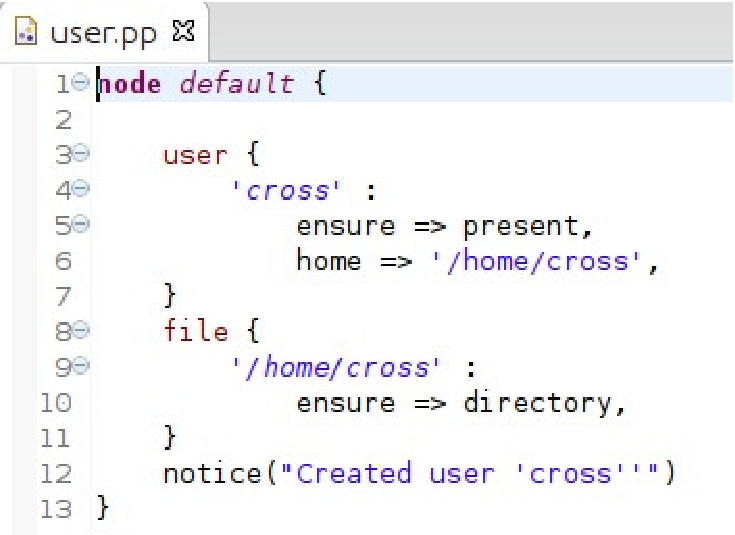
\includegraphics[width=0.7\textwidth]{images/user.pdf}
  \end{center}
  \caption{User mit Puppet anlegen}
  \label{puppet-user}
\end{figure}

\section{Autoren}

\begin{table}
\begin{tabular}{|p{0.5\textwidth}|p{0.5\textwidth}|}
\hline
Anders Malmborg
&
Michael Haslgrübler
\\
\hline
\end{tabular}
\end{table}

\bibliographystyle{apalike2}
\bibliography{document}

\end{document}
